\documentclass{standalone}

\usepackage{tikz}
\usepackage{xcolor}
\definecolor{primary}{HTML}{003262} % berkeley blue
\definecolor{secondary}{HTML}{FDB515} % cal gold
\definecolor{founder}{HTML}{3B7EA1}
\definecolor{medalist}{HTML}{C4820E}
\definecolor{goldengate}{HTML}{ED4E33}
\definecolor{ion}{HTML}{CFDD45}

\begin{document}
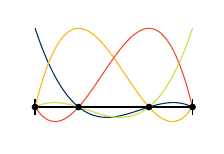
\begin{tikzpicture}
	% \tikzset{shift=(current page.center), xshift=-4cm, yshift=-3.75cm}
	\scriptsize
	\draw (0,-.1) grid[step=2] (2,.1); 
	\draw[domain=0:2, smooth, primary] plot 
		(\x, 1. - 3.*\x + 2.5*\x^2 - 0.625*\x^3); 
	\draw[domain=0:2, smooth, secondary] plot 
		(\x, 0.+4.04508*\x-4.81763*\x^2+1.39754*\x^3); 
	\draw[domain=0:2, smooth, goldengate] plot 
		(\x, 0.-1.54508*\x+3.56763*\x^2-1.39754*\x^3); 
	\draw[domain=0:2, smooth, ion] plot
		(\x, 0.+0.5*\x-1.25*\x^2+0.625*\x^3); 
	\foreach \x in {0,.552786, 1.44721,2}{
		\filldraw[black] (\x,0) circle[radius=1pt]; 
	}
	\node at (0,-.15) {}; 
\end{tikzpicture}
\end{document}